\pagestyle{fancy}
\setlength{\headheight}{16pt}
\fancyhead{} % clear all header fields
\fancyhead[L]{\textbf{CEE 576 Homework 1}}
\fancyhead[C]{Songyuan Cui}
\fancyhead[R]{\textbf{Fall 2024}}
\fancyfoot{} % clear all footer fields
\fancyfoot[C]{\thepage}

\noindent \emph{Disclaimer}. All computer programs in this assignment are implemented in \matlab~and can be found at \url{https://github.com/sy-cui/CSE552-FA2024/tree/main/homework/hw1}. 
The codes are tested in \matlab~version 2024a. 
However, latest \matlab~features are intentially avoided to maximize backward-compatibility, so the code should work out-of-the-box in most \matlab~versions. 
The directory is self-containing and does not dependent on external programs or packages. 
However, please make sure to copy \emph{the entire directory} as there are functions defined in individual files that are used by other files. 


\section{Newton-Raphson convergence}
Here we assume the algebraic error convergence recurrence formula 
\begin{equation}\label{eqn:hw1_p1_error}
    \| e_{n+1} \| \leq C \| e_n \|^k.
\end{equation}
where for simplicity we take equality. 
Given an initial error of $0.9$, the iterations taken to reach $\| e_n \| \leq 0.036$ are shown in \cref{tab:hw1_p1_error}.
For $C=1$, $k=1.1$, $37$ iterations are needed to bring the error below $0.036$, while for $C=0.5$, $k=1$ only $5$ are needed. 

\begin{table}[!ht]
    \centering
    \begin{tabular}{|c|c|c|c|}
        \hline
        \multicolumn{2}{|c|}{$C=1$, $k=1.1$} & \multicolumn{2}{|c|}{$C=0.5$, $k=1$} \\
        \hline
        $n$ & $ \|e_n \| $ & $n$ & $\|e_n \|$ \\
        \hline
        0 & 0.9 & 0 & 0.9 \\
        \hline 
        1 & 0.8905673324 & 1 & 0.45 \\
        \hline 
        2 & 0.8803055429 & 2 & 0.225 \\
        \hline 
        3 & 0.8691540938 & 3 & 0.1125 \\
        \hline 
        4 & 0.8570505897 & 4 & 0.05625 \\
        \hline 
        5 & 0.8439313183 & \textcolor{red}{5} & \textcolor{red}{0.028125} \\
        \hline 
          & \ldots & 6 & 0.0140625 \\
        \hline 
        33 & 0.08655162295 & 7 & 0.00703125 \\
        \hline 
        34 & 0.06776457789 & 8 & 0.003515625 \\
        \hline 
        35 & 0.05177296187 & 9 & 0.0017578125 \\
        \hline 
        36 & 0.03850466172 & 10 & 0.00087890625 \\
        \hline 
        \textcolor{red}{37} & \textcolor{red}{0.02780127051} & 11 & 0.000439453125 \\
        \hline 
    \end{tabular}
    \caption{
        Error evolution based on \cref{eqn:hw1_p1_error}. Iterations where errors drop below $0.036$ are marked in red. 
        For conciseness, iterations 6--32 are omitted for $C = 1$, $k = 1.1$.
    }
    \label{tab:hw1_p1_error}
\end{table}

\section{Bar structure calculation}
The following parameters are given for this problem:
\begin{equation}
    L_a = \qty{10}{\centi\meter}, ~~ L_b = \qty{5}{\centi\meter}, ~~ A = \qty{1}{\centi\meter\squared}, ~~ E_e = \qty[per-mode=symbol]{1e+7}{\newton\per\centi\meter\squared}, ~~ E_p = \qty[per-mode=symbol]{1e+5}{\newton\per\centi\meter\squared}, ~~ \varepsilon_y = 2\times 10^{-3}
\end{equation}
where $L_a$ and $L_b$ are the left and right segment length, $A$ is the uniform cross-sectional area, $E_e$ and $E_p$ are the Young's modulus for the elastic and plastic regimes respectively, and $\epsilon_y$ is the yielding strain. 
This leads to a nonlinear consitutive relation which can be written as 
\begin{equation}
    \sigma(\varepsilon) = \begin{cases}
        E_e \varepsilon, & \textrm{if} ~~\varepsilon \leq \varepsilon_y \\
        E_e \varepsilon_y + E_p(\varepsilon - \varepsilon_y), & \textrm{if} ~~\varepsilon > \varepsilon_y
    \end{cases}
\end{equation}
An external force $F^{\textrm{ext}}$ is imposed at the intersection between segments $A$ and $B$, causing an unknown displacement $u$. 
The force balance at this point can be cast as a nonlinear problem of the form 
\begin{equation}\label{eqn:hw1_p2_fint}
    F^{\textrm{int}}(u) = \left[\sigma\left(\frac{u}{L_a}\right) + \sigma\left(\frac{u}{L_b}\right)\right] A = F^{\textrm{ext}}.
\end{equation}
Given the displacement and residual at the current iteration $u^{(i)}$ and $r^{(i)}$, the tangent operator $K$ (obtained at the start of the load for modified Newton's method), and the current external load $F^{\textrm{ext}}$, the iteration step is summarized as 
\begin{subequations}
\begin{equation}\label{eqn:hw1_p2_du}
    \Delta u^{(i)} = K^{-1} r^{(i)}
\end{equation}
\begin{equation}\label{eqn:hw1_p2_u_update}
    u^{(i+1)} = u^{(i)} + \Delta u^{(i)}
\end{equation}
\begin{equation}\label{eqn:hw1_p2_r_update}
    r^{(i+1)} = F^{\textrm{ext}} - F^{\textrm{int}}(u^{(i+1)})
\end{equation}
\end{subequations}
% The convergence of modified Newton-Raphson iterations is determined based on the relative residual functionally represented as 
% \begin{equation*}
%     \tilde{r}^{(i)}:= \frac{r^{(i)}}{r^{(0)}} \leq \epsilon ~~~~ \Leftrightarrow ~~~~ r^{(i)} \leq \epsilon r^{(0)}
% \end{equation*}
% where $r^{(0)}$ is the initial residual at the start of the load step. 

For the second load step ($F_2^{\textrm{ext}} = \qty{4e+4}{\newton}$), the modifed Newton-Raphson method uses the same tangent operator $K_2 = \qty[per-mode=symbol]{3e+6}{\newton\per\centi\meter}$. 
An absolute tolerance of $\epsilon = \qty{0.1}{\newton}$ is used (for residuals). 
The first iteration leads to displacement $u_2^{(1)} \approx \qty{1.3333e-2}{\centi\meter}$ and residual $r_2^{(1)} = \qty{6600}{\newton}$.
The second iteration leads to displacement $u_2^{(2)} \approx \qty{1.5533e-2}{\centi\meter}$ and residual $r_2^{(2)} = \qty{4356}{\newton}$.
Here, we explicitly use ``$=$'' for exact results and ``$\approx$'' for truncated results.
At this iteration, bar $A$ is elastic while bar $B$ is plastic. 


\emph{Iteration 3.} The incremental displacement can be evaluated using \cref{eqn:hw1_p2_du} as 
\begin{equation*}
    \Delta u^{(2)} = K_2^{-1} r_2^{(2)} = \frac{\qty{4356}{\newton}}{\qty[per-mode=symbol]{3e+6}{\newton\per\centi\meter}} = \qty{1.452e-3}{\centi\meter}.
\end{equation*}
The new displacement is then (\cref{eqn:hw1_p2_u_update})
\begin{equation*}
    u_2^{(3)} = u_2^{(2)} + \Delta u^{(2)} \approx \qty{1.5533e-2}{\centi\meter} +  \qty{1.452e-3}{\centi\meter} \approx \qty{1.6985e-2}{\centi\meter}.
\end{equation*}
The new residual, using \cref{eqn:hw1_p2_r_update,eqn:hw1_p2_fint}, is calculated as 
\begin{equation*}
    r_2^{(3)} = F_2^{\textrm{ext}} - F^{\textrm{int}}(u_2^{(3)}) \approx \qty{4e+4}{\newton} - \qty{3.7125e+4}{\newton} = \qty{2874.96}{\newton},
\end{equation*}
which is larger than the absolute tolerance $\epsilon = \qty{0.1}{\newton}$, suggesting more iterations are required. 

\emph{Iteration 4.} The incremental displacement can be evaluated using \cref{eqn:hw1_p2_du} as 
\begin{equation*}
    \Delta u^{(3)} = K_2^{-1} r_2^{(3)} = \frac{\qty{2874.96}{\newton}}{\qty[per-mode=symbol]{3e+6}{\newton\per\centi\meter}} \approx \qty{9.5832e-4}{\centi\meter}.
\end{equation*}
The new displacement is then (\cref{eqn:hw1_p2_u_update})
\begin{equation*}
    u_2^{(4)} = u_2^{(3)} + \Delta u^{(3)} \approx \qty{1.6985e-2}{\centi\meter} +  \qty{9.5832e-4}{\centi\meter} \approx \qty{1.7944e-2}{\centi\meter}.
\end{equation*}
The new residual, using \cref{eqn:hw1_p2_r_update,eqn:hw1_p2_fint}, is calculated as 
\begin{equation*}
    r_2^{(4)} = F_2^{\textrm{ext}} - F^{\textrm{int}}(u_2^{(4)}) \approx \qty{4e+4}{\newton} - \qty{3.8103e+4}{\newton} \approx \qty{1897.47}{\newton},
\end{equation*}
which is larger than the absolute tolerance $\epsilon = \qty{0.1}{\newton}$, suggesting more iterations are required. 

Key outputs of the the rest of the modifed Newton-Raphson iterations are given below. A total of 28 iterations are required for the residual magnitude $\| r_2^{(k)}\|$ to drop below $\epsilon = \qty{0.1}{\newton}$.
The final solution is $u_2 \approx \qty{0.01980}{\centi\meter}$, with bar $A$ still in the elastic regime and bar $B$ in the plastic regime. 

\begin{codenv}{Modified Newton-Raphson iterations at the second load step}
\indent iter=0, K=3e+06, u=6.666667e-03, Fint=2.000000e+04, res=2.000000e+04, du=6.666667e-03

iter=1, K=3e+06, u=1.333333e-02, Fint=3.340000e+04, res=6.600000e+03, du=2.200000e-03

iter=2, K=3e+06, u=1.553333e-02, Fint=3.564400e+04, res=4.356000e+03, du=1.452000e-03

iter=3, K=3e+06, u=1.698533e-02, Fint=3.712504e+04, res=2.874960e+03, du=9.583200e-04

iter=4, K=3e+06, u=1.794365e-02, Fint=3.810253e+04, res=1.897474e+03, du=6.324912e-04

iter=5, K=3e+06, u=1.857614e-02, Fint=3.874767e+04, res=1.252333e+03, du=4.174442e-04

iter=6, K=3e+06, u=1.899359e-02, Fint=3.917346e+04, res=8.265395e+02, du=2.755132e-04

iter=7, K=3e+06, u=1.926910e-02, Fint=3.945448e+04, res=5.455161e+02, du=1.818387e-04

iter=8, K=3e+06, u=1.945094e-02, Fint=3.963996e+04, res=3.600406e+02, du=1.200135e-04

iter=9, K=3e+06, u=1.957095e-02, Fint=3.976237e+04, res=2.376268e+02, du=7.920893e-05

iter=10, K=3e+06, u=1.965016e-02, Fint=3.984317e+04, res=1.568337e+02, du=5.227790e-05

iter=11, K=3e+06, u=1.970244e-02, Fint=3.989649e+04, res=1.035102e+02, du=3.450341e-05

iter=12, K=3e+06, u=1.973694e-02, Fint=3.993168e+04, res=6.831675e+01, du=2.277225e-05

iter=13, K=3e+06, u=1.975972e-02, Fint=3.995491e+04, res=4.508906e+01, du=1.502969e-05

iter=14, K=3e+06, u=1.977475e-02, Fint=3.997024e+04, res=2.975878e+01, du=9.919593e-06

iter=15, K=3e+06, u=1.978467e-02, Fint=3.998036e+04, res=1.964079e+01, du=6.546931e-06

iter=16, K=3e+06, u=1.979121e-02, Fint=3.998704e+04, res=1.296292e+01, du=4.320975e-06

iter=17, K=3e+06, u=1.979553e-02, Fint=3.999144e+04, res=8.555530e+00, du=2.851843e-06

iter=18, K=3e+06, u=1.979839e-02, Fint=3.999435e+04, res=5.646650e+00, du=1.882217e-06

iter=19, K=3e+06, u=1.980027e-02, Fint=3.999627e+04, res=3.726789e+00, du=1.242263e-06

iter=20, K=3e+06, u=1.980151e-02, Fint=3.999754e+04, res=2.459681e+00, du=8.198935e-07

iter=21, K=3e+06, u=1.980233e-02, Fint=3.999838e+04, res=1.623389e+00, du=5.411297e-07

iter=22, K=3e+06, u=1.980287e-02, Fint=3.999893e+04, res=1.071437e+00, du=3.571456e-07

iter=23, K=3e+06, u=1.980323e-02, Fint=3.999929e+04, res=7.071483e-01, du=2.357161e-07

iter=24, K=3e+06, u=1.980346e-02, Fint=3.999953e+04, res=4.667179e-01, du=1.555726e-07

iter=25, K=3e+06, u=1.980362e-02, Fint=3.999969e+04, res=3.080338e-01, du=1.026779e-07

iter=26, K=3e+06, u=1.980372e-02, Fint=3.999980e+04, res=2.033023e-01, du=6.776744e-08

iter=27, K=3e+06, u=1.980379e-02, Fint=3.999987e+04, res=1.341795e-01, du=4.472651e-08

iter=28, K=3e+06, u=1.980383e-02, Fint=3.999987e+04, res=8.855849e-02, du=4.472651e-08

\end{codenv}

\section{Bar structure computation}
Following the previous problem, the nonlinear equation \cref{eqn:hw1_p2_fint} can be solved via either the Newton-Raphson (N-R) method or the Modified Newton-Raphson (M-N-R) method. 
The general algorithm for these approaches are listed in \cref{alg:hw1_nr,alg:hw1_mnr}, respectively. 
A representitive flow chart is shown in \cref{fig:hw1_flow_chart}.
We note that the external loads are applied in incremental load steps denoted in \emph{subscripts}, while the paranthesized \emph{superscripts} correspond to Newton iterations.
For example, $u_n^{(k)}$ represent the $k$-th iteration during the $n$-th load step. 

The two algorithms are largely identical, with the only difference in where the consistent tangent is computed (marked in \textcolor{Maroon}{dark red}).
The N-R method compute the consistent tangent at every iteration, while M-N-R do this only at the start of a load step and the same tangent is used throughout the step. 

Numerical implementation of both N-R and M-N-R is accomplished in \matlab. 
The force-displacement curve, with two successive load steps $F^{\textrm{ext}}_1 = \qty{2e+4}{\newton}$ and $F^{\textrm{ext}}_2 = \qty{4e+4}{\newton}$, is shown in \cref{fig:hw1_p3_fd}.
To achieve an absolute tolerance of $\qty{e-12}{\newton}$, N-R requires \emph{2} iterations in both the first load step and the second, while M-N-R requires \emph{2} iteartions in the first step and \emph{85} iterations in the second.
We note that in the first load step, both approaches should yield the exact solution after exactly one iteration as plasticity has not set in at this step, but 2 iterations are observed. 
This is due to round-off error amplified by poor conditioning, and can be (significantly) mitigated by introducing relative errors. 

The history of residual for N-R is 
\begin{align*}
    \textrm{Load step 1}: &~~ \qty{2e+4}{\newton} &\rightarrow& ~~ \qty{-3.673e-12}{\newton}~(\textrm{round-off}) &\rightarrow ~~ 0 \\
    \textrm{Load step 2}: &~~ \qty{2e+4}{\newton} &\rightarrow& ~~ \qty{6600}{\newton} &\rightarrow ~~ 0 \\
\end{align*}
and for M-N-R, the first load step is \emph{exactly the same as N-R}, as their consistent tangents are identical. 
The second load step involves 85 iterations and the residual reduction is hence not tabulated, instead shown in \cref{fig:hw1_p3_fd} (right) which \emph{decays exponentially} with the number of M-N-R iterations. 

Comparing N-R and M-N-R, it is immediately obvious that \emph{M-N-R takes significantly more iterations to converge to the same tolerance}.
However, M-N-R also does not require the re-evaluation of the consistent tangent at every step. 
Timing the two approaches in this problem reveal that N-R is in general $50\%$ faster to converge than M-N-R.
However, it should be noted that this disparity is not representitive as this is only a scalar problem.
In nonlinear finite element formulations, the cost of re-computing (and potentially factorizing) the consistent tangent in N-R may become much more taxing. On the other hand, M-N-R enjoys the benefit of acceleration techniques and opportunity to be pre-factorizated, rendering it the potentially more appealing approach. 
\begin{figure}[!ht]
    \centering
    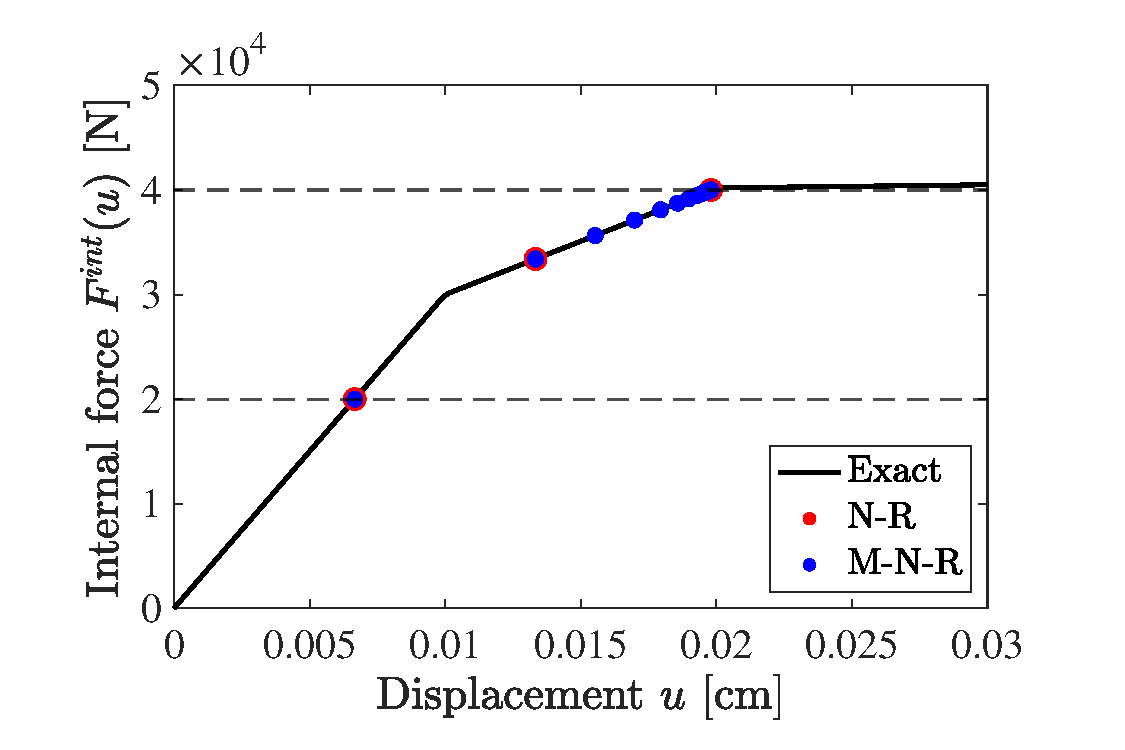
\includegraphics[width=\linewidth]{homework/hw1/hw1_p3.pdf}
    \caption{Exact force-displacement curve and computation results using N-R (red dots) and M-N-R (blue dots) iterations are shown on the left. 
    The plot on the right shows the residual reduction for M-N-R in the second load step. }
    \label{fig:hw1_p3_fd}
\end{figure}

\section{Differentiable nonlinear problem}
\subsection*{Part A}
We now consider the nonlinear problem 
\begin{equation}\label{eqn:hw1_p4_nlp}
    F^{\textrm{int}}(u) = (0.19u^3 - 2u^2 + 6u + 0.1)e^{0.02u} = F^{\textrm{ext}}
\end{equation}
All algorithms \cref{alg:hw1_nr,alg:hw1_mnr} (and flow charts \cref{fig:hw1_flow_chart}) described in the preceding problem can still be applied here. 
With incremental load steps from \qty{0}{\newton} to \qty{5.5}{\newton} at \qty{0.5}{\newton} intervals and an absolute tolerance of $\epsilon = \qty{e-12}{\newton}$, the required number of iterations are tabulated in \cref{tab:hw1_p4_iters}, and results are plotted in \cref{fig:hw1_p4_fd}.
For simplicity, we do not tabulate here the numerical values of the residual of every iteration. 
Instead, the concatenated residuals for all load steps for both N-R and M-N-R iterations are plotted in \cref{fig:hw1_p4_res}.

\begin{table}[!ht]
\centering
\begin{tabular}{|c|c|c|c|}
    \hline
    Load steps $n$ & $F^{\textrm{ext}}_n$ [\si{\newton}] & N-R iterations & M-N-R iterations \\
    \hline 
    1 & 0.5 & 3 & 9 \\ 
    \hline 
    2 & 1.0 & 4 & 10 \\ 
    \hline 
    3 & 1.5 & 4 & 10 \\ 
    \hline 
    4 & 2.0 & 4 & 10 \\ 
    \hline 
    5 & 2.5 & 4 & 11 \\ 
    \hline 
    6 & 3.0 & 4 & 11 \\ 
    \hline 
    7 & 3.5 & 4 & 12 \\ 
    \hline 
    8 & 4.0 & 4 & 13 \\ 
    \hline 
    9 & 4.5 & 4 & 15 \\ 
    \hline 
    10 & 5.0 & 4 & 18 \\ 
    \hline 
    11 & 5.5 & 5 & 26 \\ 
    \hline
\end{tabular}
\caption{Number of iterations required for N-R and M-N-R in each load step to reach the tolerance $\epsilon$. }
\label{tab:hw1_p4_iters}
\end{table}
\begin{figure}[!ht]
    \centering
    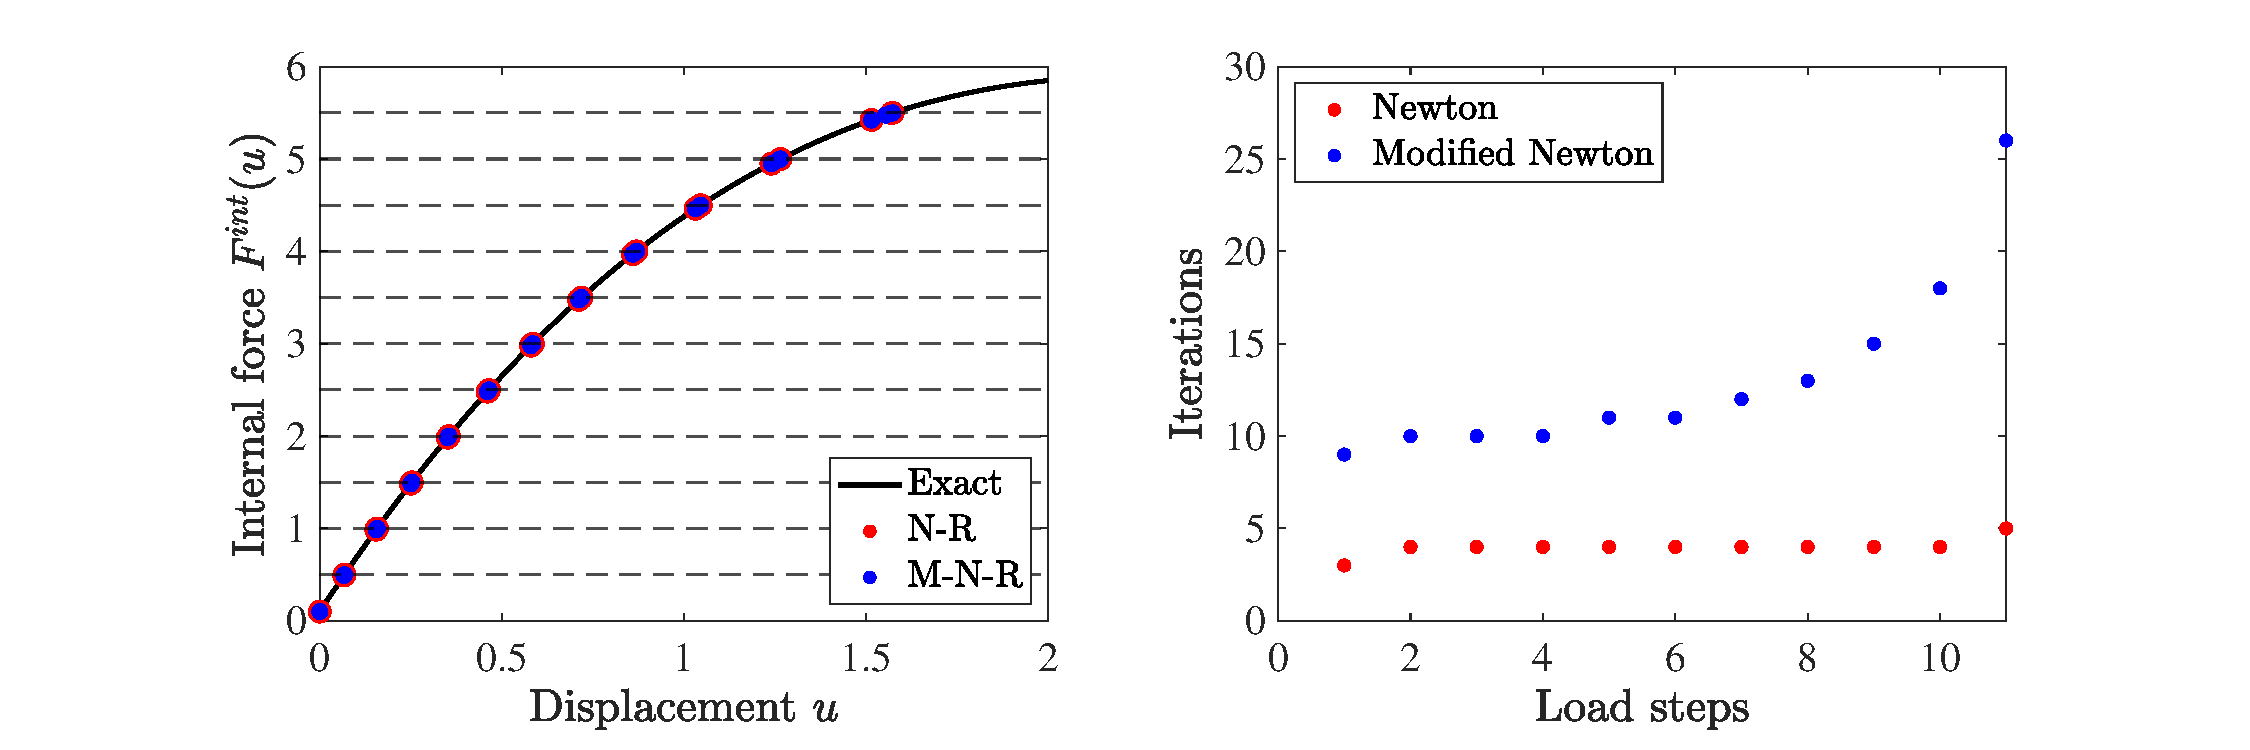
\includegraphics[width=\linewidth]{homework/hw1/hw1_p4.pdf}
    \caption{The left plot shows the exact force-displacement curve and computation results for \cref{eqn:hw1_p4_nlp} using N-R (red dots) and M-N-R (blue dots) iterations.
    The number of iterations required for both of these methods to reach $\epsilon = \qty{e-12}{\newton}$ is shown in the plot on the right. 
    }
    \label{fig:hw1_p4_fd}
\end{figure}

\subsection*{Part B}
The simulation data suggests that both the Newton-Raphson and modified Newton-Raphson algorithms converge exponentially, while N-R having about twice the exponent than M-N-R.
This reflects the fact that N-R is quadratically convergent in the context of iterative solution techiniques, while M-N-R is only linearly convergent. 
Both approaches have their benefits (and conversely drawbacks), with N-R using significantly less iterations and M-N-R not having to recompute the consistent tangent at every step. 
For every large systems with complex sources of nonlinearity, the cost of computing the consistent tangent matrix in N-R may become crippling for the overall performance. 
In such cases, it may be more computationally efficient to utilize some accelerated M-N-R techniques or a combination of the two methods. 

\begin{figure}[!ht]
    \centering
    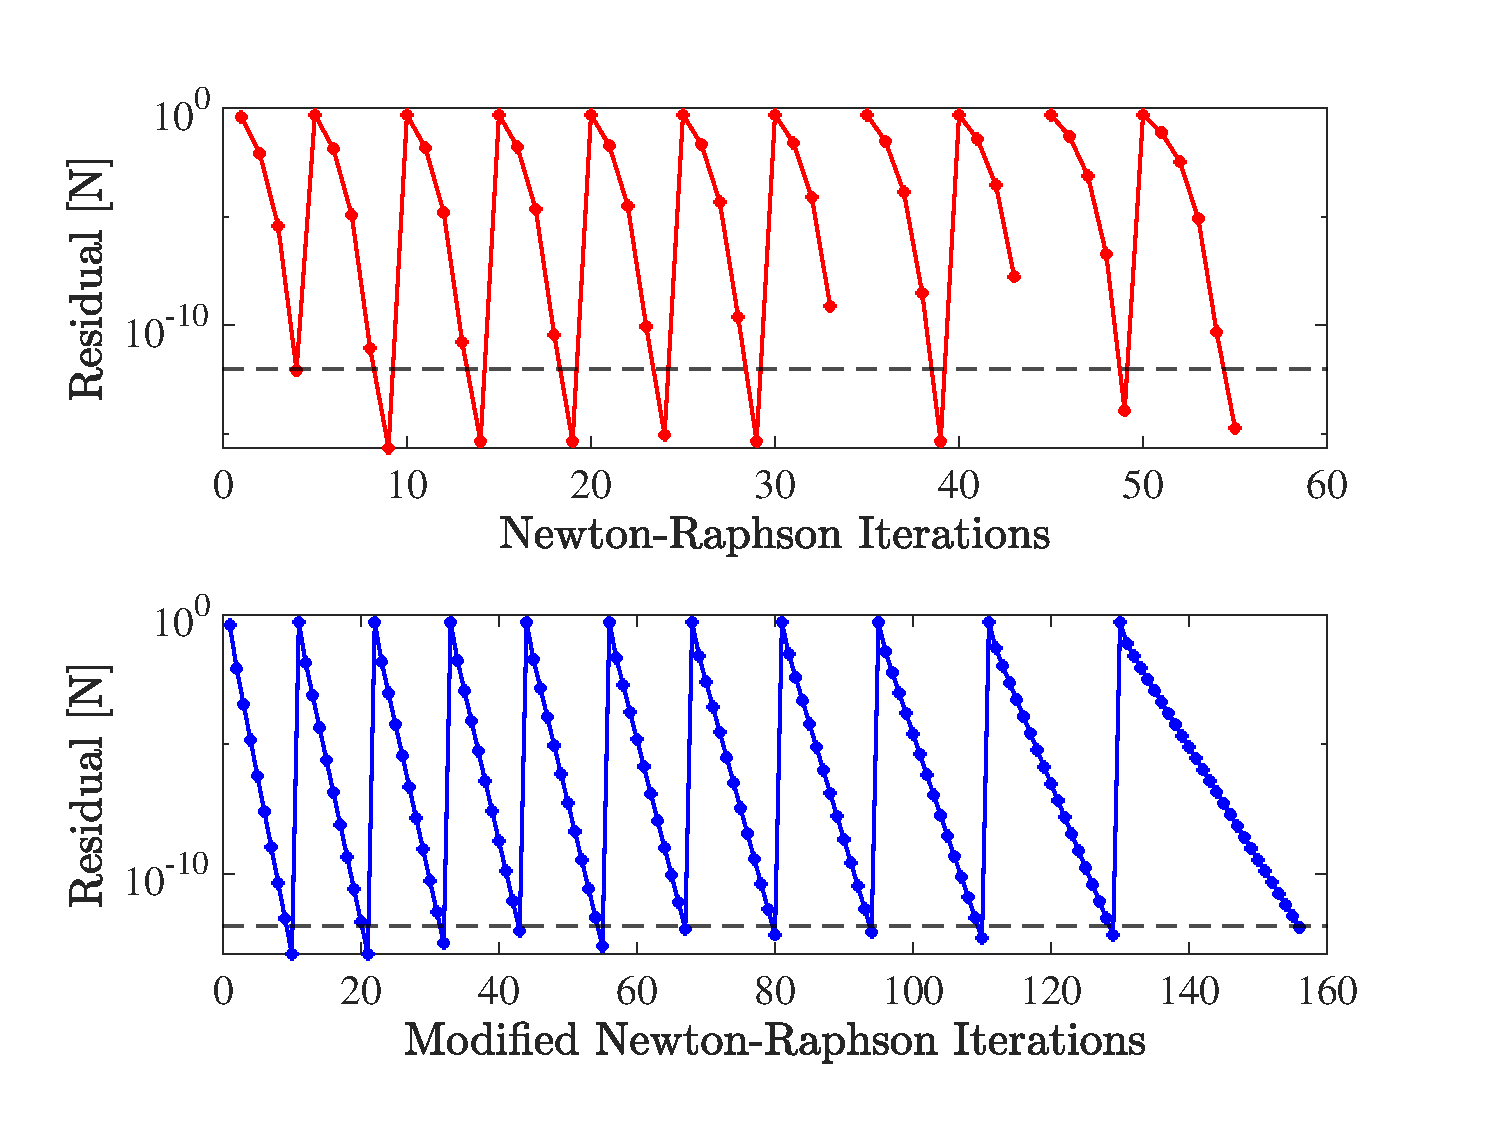
\includegraphics[width=\linewidth]{homework/hw1/hw1_p4_res.pdf}
    \caption{Residual reduction with respect to numbers of iterations for both N-R (top) and M-N-R (bottom) iterations.  
    }
    \label{fig:hw1_p4_res}
\end{figure}

\clearpage
\begin{algorithm}[!ht]
\caption{Nonlinear solution procedure with Newton-Raphson iteration}
\begin{algorithmic}\label{alg:hw1_nr}
    \setlength{\lineskip}{4pt}
    \Require{Nonlinear function $F^{\textrm{int}}(u)$, incremental load steps $F^{\textrm{ext}}_n$, Initial guess $u_0$, Tolerance $\epsilon$}
    \Ensure{Approximated solutions such that $F^{\textrm{int}}(u_n) \approx F^{\textrm{ext}}_n$}

    \For{$n = 1, 2, \ldots, N$}
    \Comment{New load step}

    \State{$u_n^{(0)} \gets u_{n-1}$}
    \Comment{Inherit solution from previous step}

    \State{$r_n^{(0)} \gets F^{\textrm{ext}}_n - F^{\textrm{int}} \left[u_n^{(0)}\right]$}
    \Comment{Compute new residual}

    \State{$k \gets 0$}

    \While{$\| r_n^{(k)}\| > \epsilon$}
        \State{\textcolor{Maroon}{$K_n^{(k)} \gets \frac{\partial}{\partial u} F^{\textrm{int}}\left[u_n^{(k)}\right]$}}
        \Comment{Compute consistent tangent}

        \State{$\Delta u_n^{(k)} = {\left[K_n^{(k)}\right]}^{-1}r_n^{(k)}$}
        \Comment{Compute incremental displacement}

        \State{$u_n^{(k+1)} \gets u_n^{(k)} + \Delta u_n^{(k)}$}
        \Comment{Update displacement}

        \State{$r_n^{(k+1)} \gets F^{\textrm{ext}}_n - F^{\textrm{int}} \left[u_n^{(k+1)}\right]$}
        \Comment{Update residual}

        \State{$k \gets k + 1$}
    \EndWhile{}

    \State{$u_n \gets u_n^{(k)}$}
    \Comment{Solution of the $n$-th load step}

    \EndFor{}
\end{algorithmic}
\end{algorithm}


\begin{algorithm}[!ht]
\caption{Nonlinear solution procedure with Modified Newton-Raphson iteration}
\begin{algorithmic}\label{alg:hw1_mnr}
    \setlength{\lineskip}{4pt}
    \Require{Nonlinear function $F^{\textrm{int}}(u)$, incremental load steps $F^{\textrm{ext}}_n$, Initial guess $u_0$, Tolerance $\epsilon$}
    \Ensure{Approximated solutions such that $F^{\textrm{int}}(u_n) \approx F^{\textrm{ext}}_n$}

    \For{$n = 1, 2, \ldots, N$}
    \Comment{New load step}

    \State{$u_n^{(0)} \gets u_{n-1}$}
    \Comment{Inherit solution from previous step}

    \State{$r_n^{(0)} \gets F^{\textrm{ext}}_n - F^{\textrm{int}} \left[u_n^{(0)}\right]$}
    \Comment{Compute new residual}

    \State{$k \gets 0$}

    \State{\textcolor{Maroon}{$K_n \gets \frac{\partial}{\partial u} F^{\textrm{int}}\left[u_n^{(0)}\right]$}}
    \Comment{Compute consistent tangent only at $k = 0$}

    \While{$\| r_n^{(k)}\| > \epsilon$}
        
        \State{$\Delta u_n^{(k)} = K_n^{-1}r_n^{(k)}$}
        \Comment{Compute incremental displacement}

        \State{$u_n^{(k+1)} \gets u_n^{(k)} + \Delta u_n^{(k)}$}
        \Comment{Update displacement}

        \State{$r_n^{(k+1)} \gets F^{\textrm{ext}}_n - F^{\textrm{int}} \left[u_n^{(k+1)}\right]$}
        \Comment{Update residual}

        \State{$k \gets k + 1$}
    \EndWhile{}

    \State{$u_n \gets u_n^{(k)}$}
    \Comment{Solution of the $n$-th load step}

    \EndFor{}
\end{algorithmic}
\end{algorithm}
\clearpage
\begin{figure}[!ht]
    \centering
    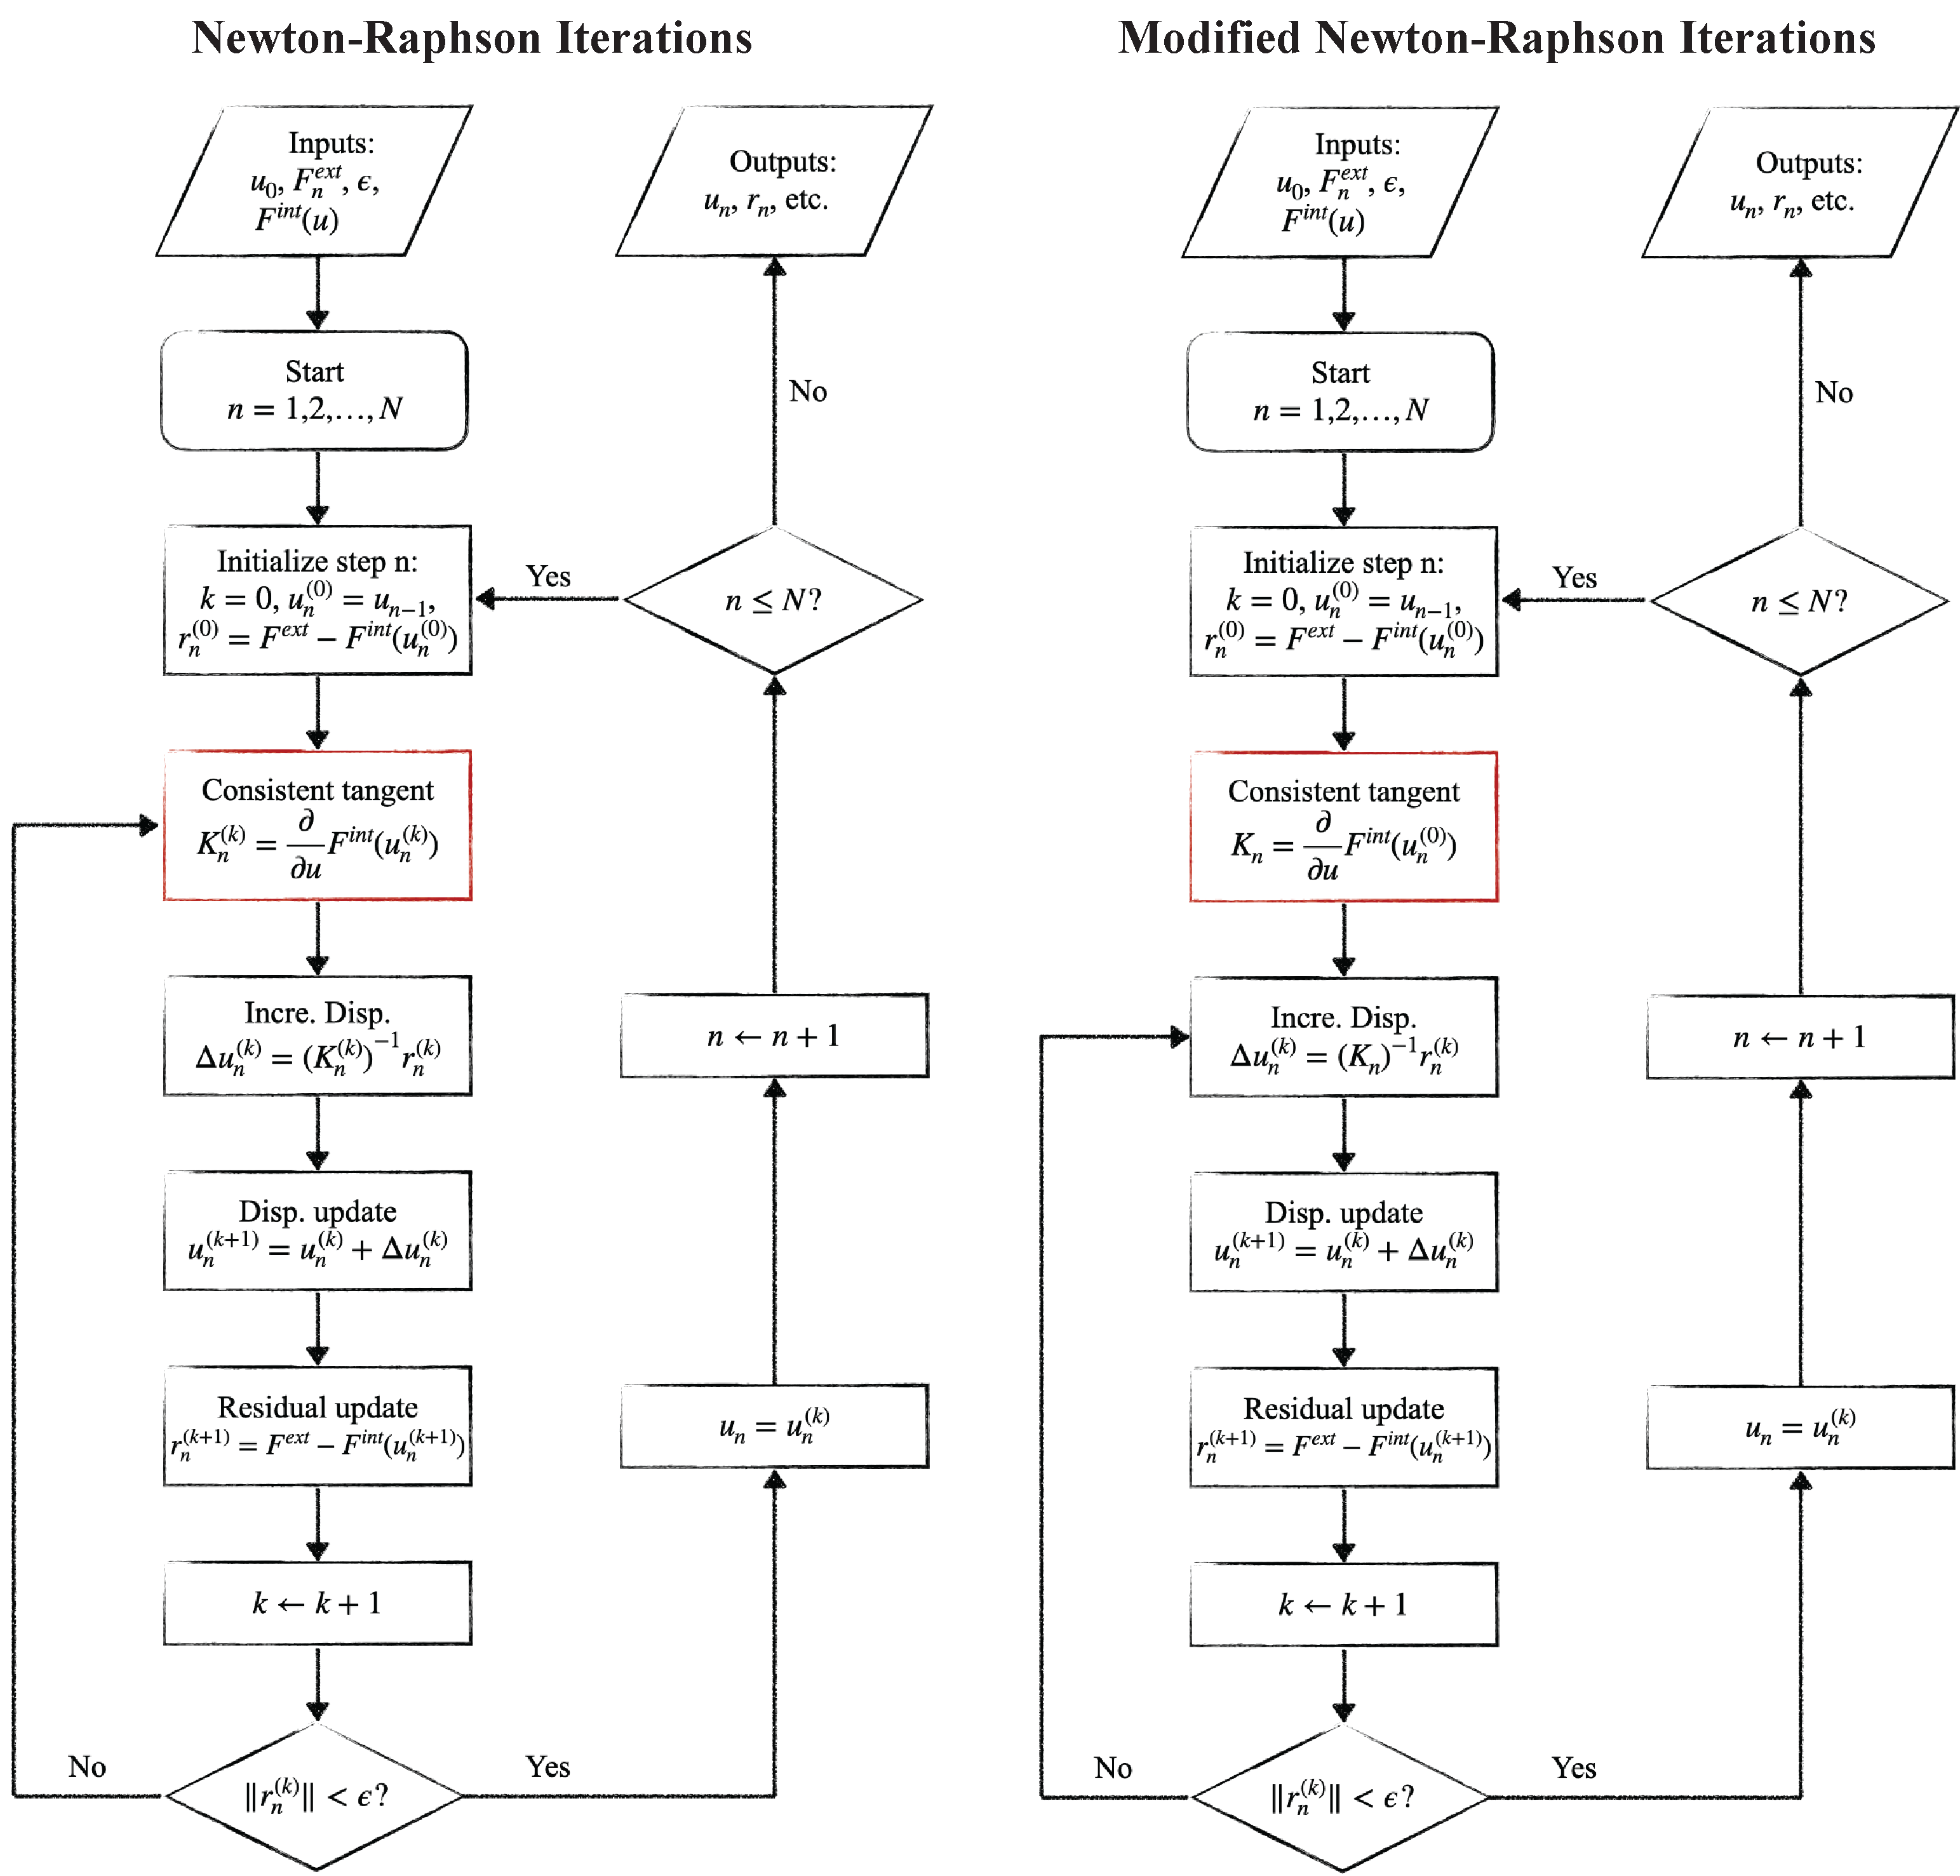
\includegraphics[width=\linewidth]{homework/hw1/hw1_flow_chart.pdf}
    \caption{Flow diagram of Newton-Raphson and modifed Newton-Raphson iterations. }
    \label{fig:hw1_flow_chart}
\end{figure}
